% Permission is granted to copy, distribute and/or modify this document
% under the terms of the GNU Free Documentation License, Version 1.2
% or any later version published by the Free Software Foundation;
% with no Invariant Sections, no Front-Cover Texts, and no Back-Cover
% Texts.  A copy of the license is included in the section entitled "GNU
% Free Documentation License".
% Copyright 2014 EDF
%


%%%%%%%%%%%%%%%%%%%%%%%%%%%%%%%%%%%%%%%%%%%%%%%%%%%%%%%%%%%%%%%%%%%%%%%%%%%%%%%%%%%%%%%%%%
\section{Validation}

This section aims at exposing the methodology used to validate numerical results of the module. The validation of \texttt{NeuralNetwork} is exposed hereafter.\\

For that purposes, the <<beam>> example, illustrated in the \texttt{ExampleGuide} documentation of \texttt{OpenTURNS}, has been choosen:
\begin{itemize}
 \item A design of experiment and the evaluation of the deviation funcion on that design were provided (\verb+input_output.dat+ file);
 \item Previous data were used to build a neural network model thanks to the \texttt{Uranie} module;
 \item The issued model (\texttt{PMML} file) is provided for validation.
\end{itemize}
In addition, the \texttt{modulePMML.py} script had been developed at EDF to parse PMML files. Thus the validation of the neural network parsing uses a script that
reads input data from \verb+input_output.dat+ file, evaluates the same PMML file with \texttt{modulePMML.py} and \texttt{OTPMLL}, gets output values, absolute and relative errors.
\lstinputlisting[language=Python]{compare_otpmml.py}

From that results, we compare in figure \ref{fig:val:outputs} outputs issued from \texttt{modulePMML.py} and \texttt{OTPMML}.\\
\begin{figure}[!h]
 \begin{center}
  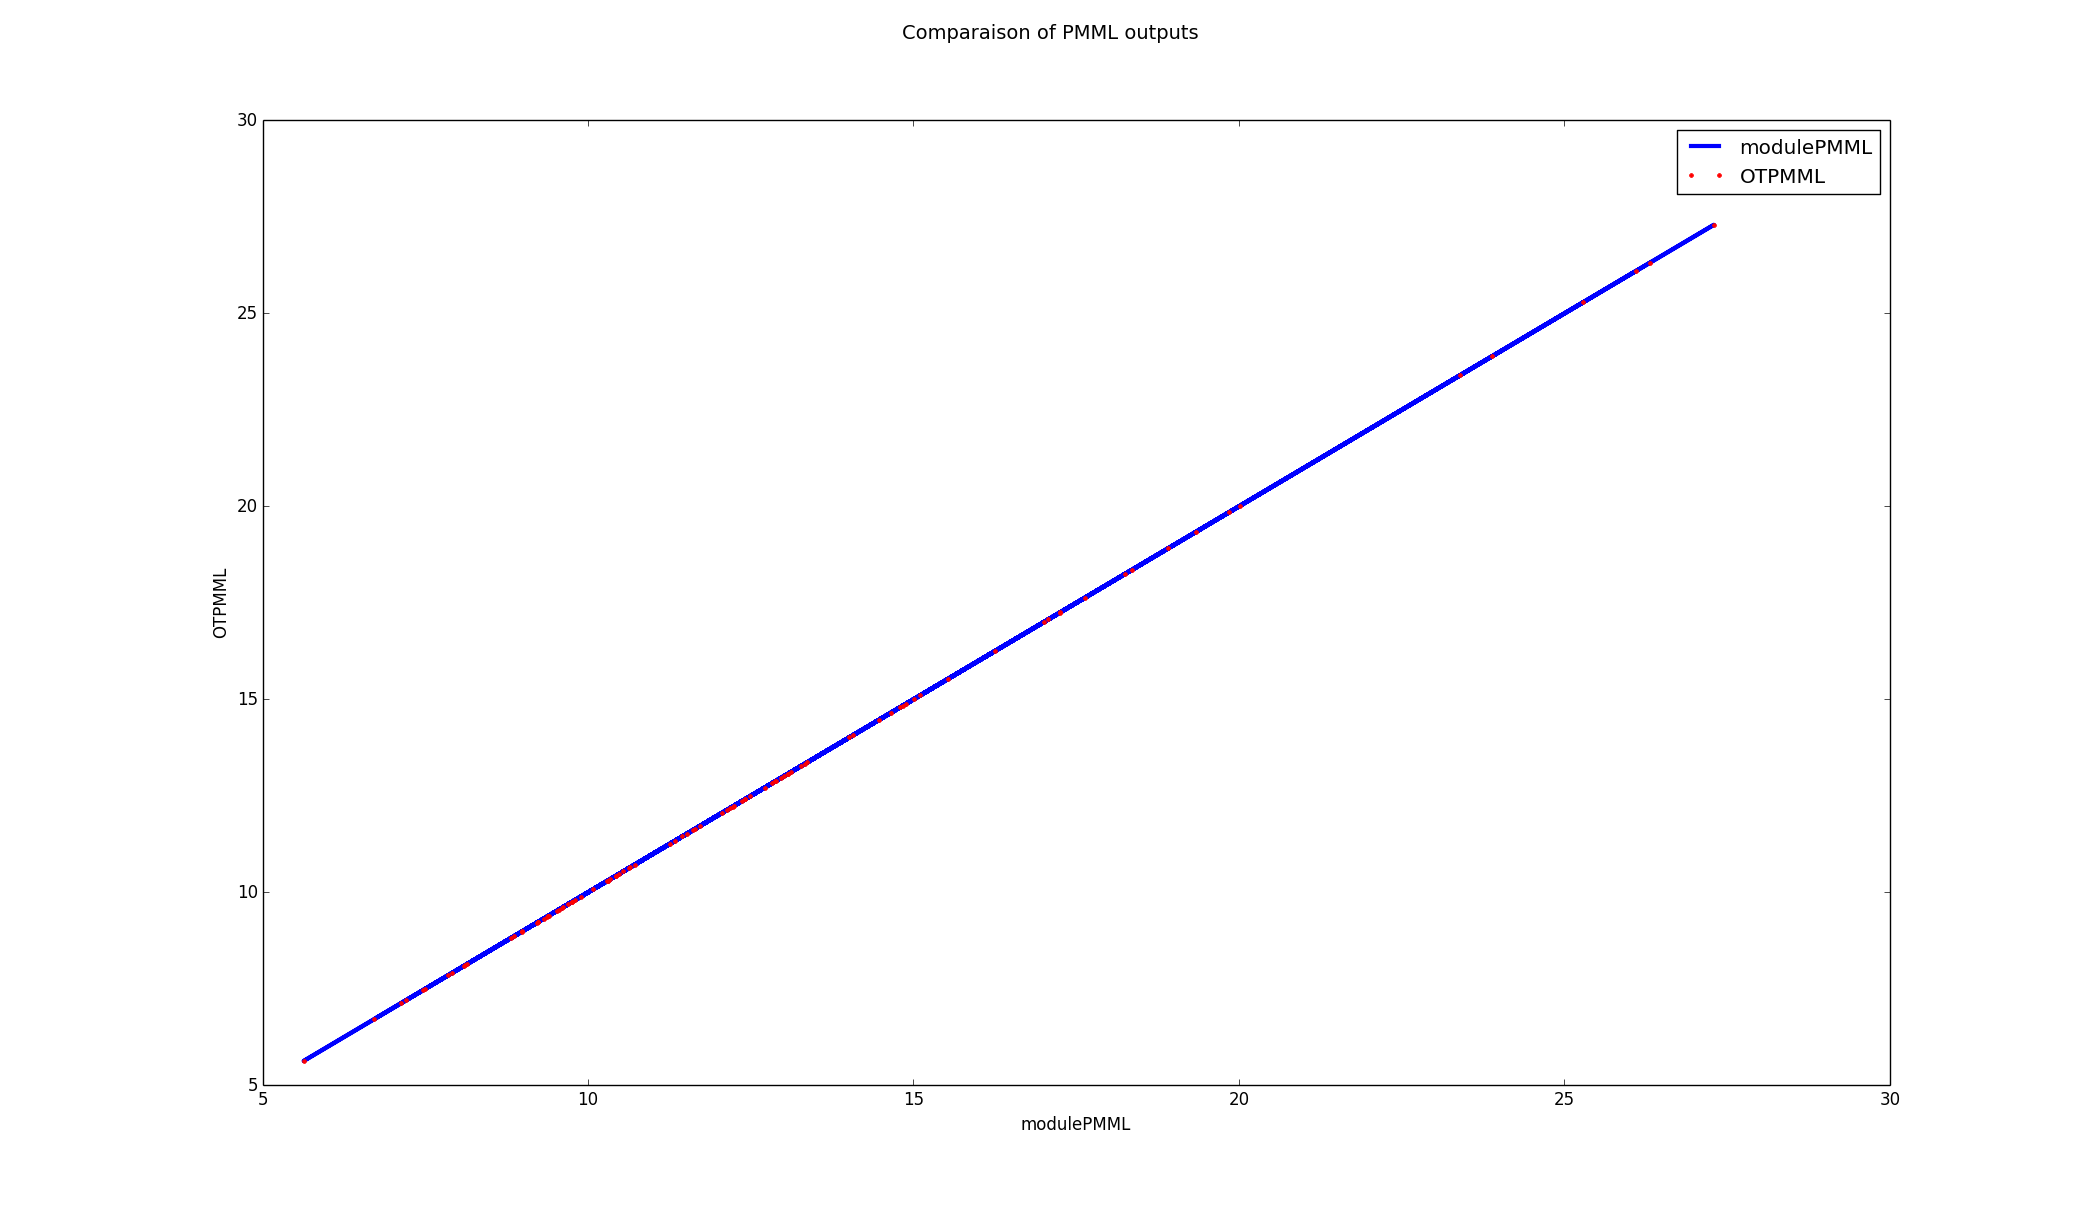
\includegraphics[scale=0.22]{comparaison_outputs.png}
 \end{center}
 \caption{Comparison of outputs}
 \label{fig:val:outputs}
\end{figure}
\newpage
In addition, errors are ploted in figure \ref{fig:val:errors}.
\begin{figure}[h]
 \begin{center}
  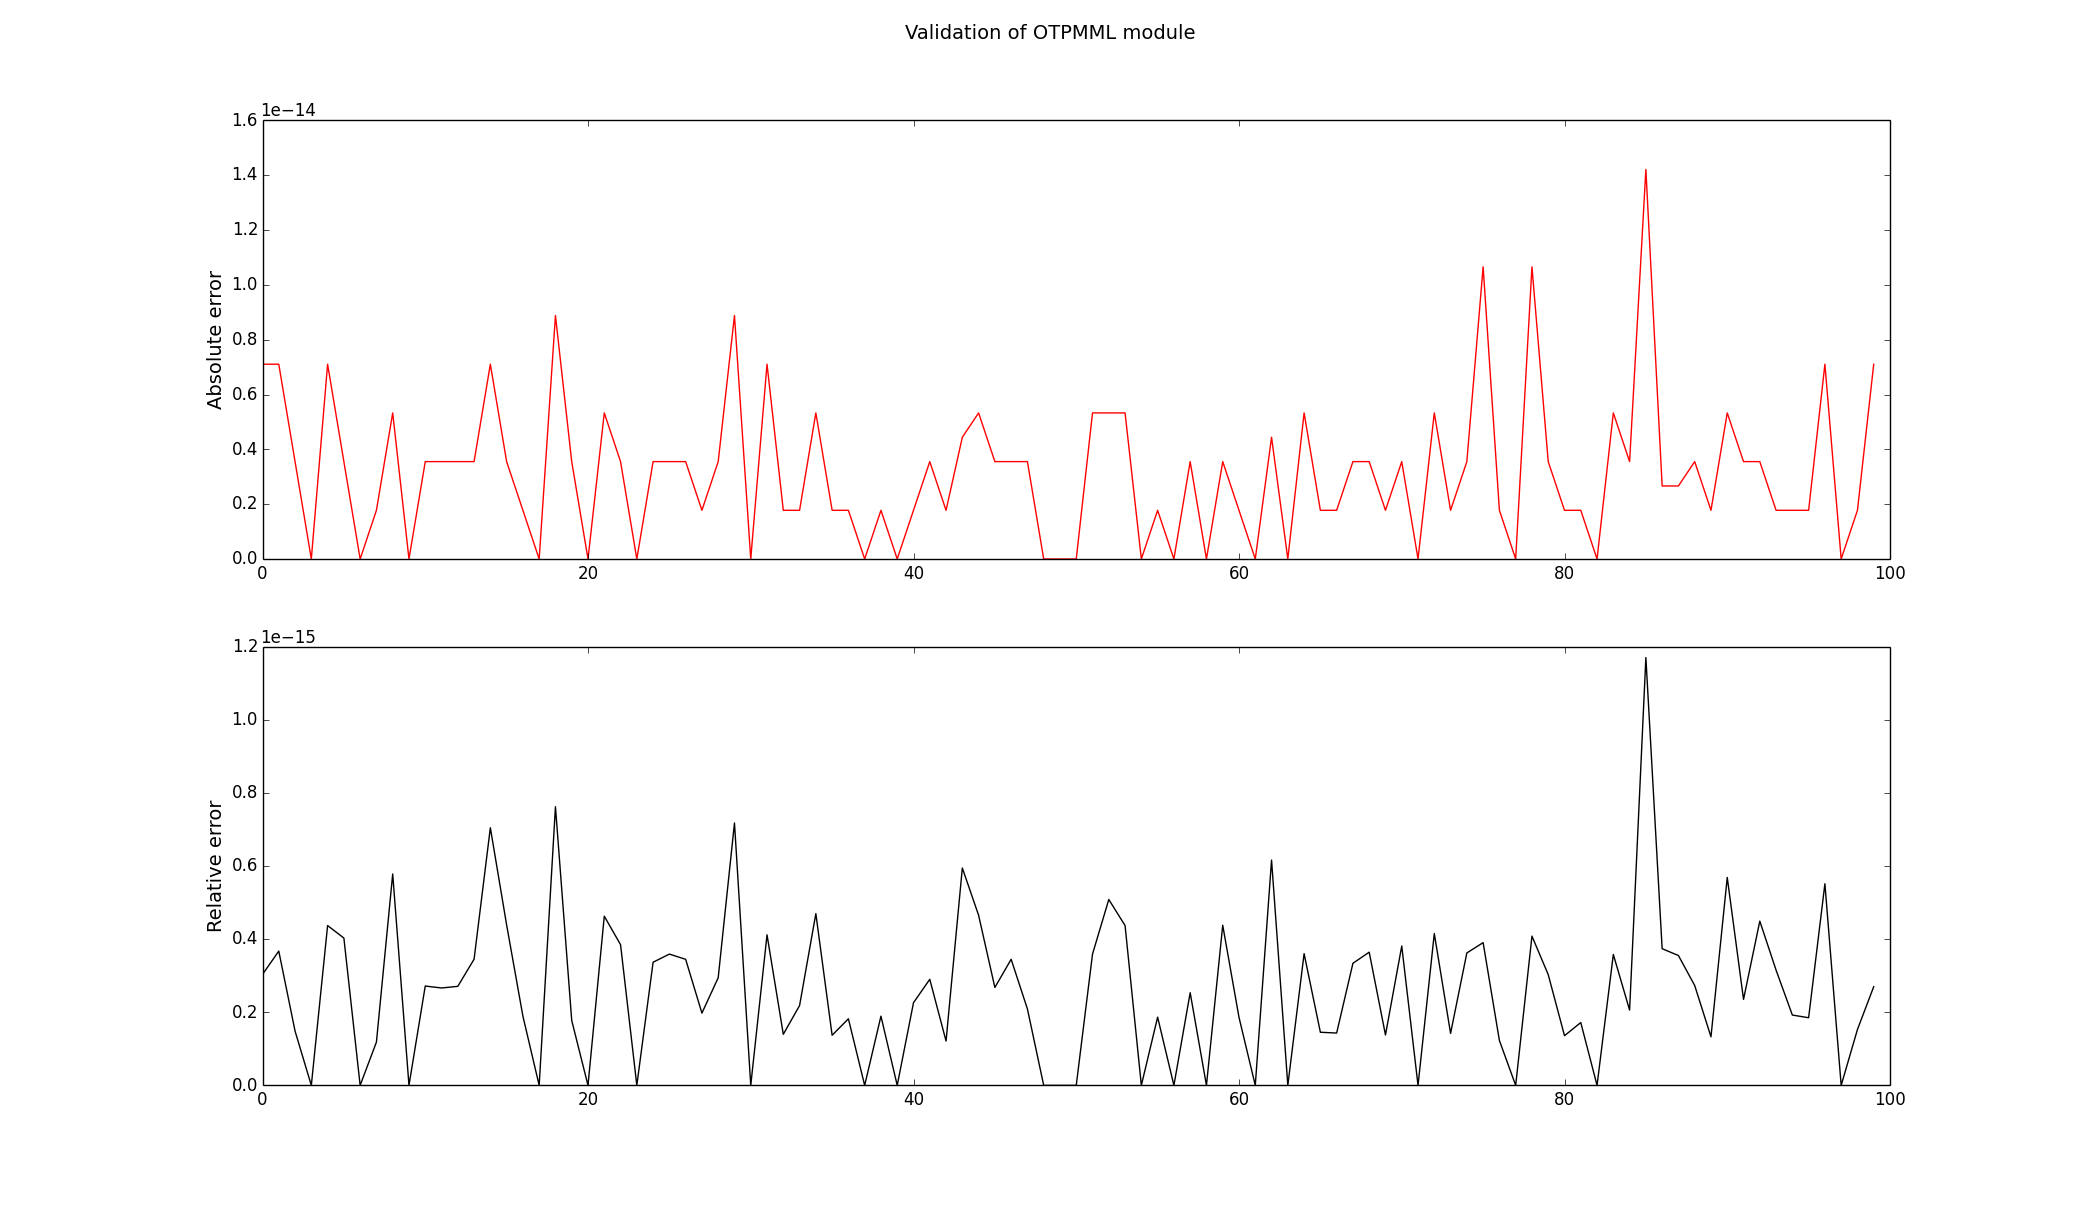
\includegraphics[scale=0.22]{absolute_relative_errors.png}
 \end{center}
 \caption{Comparison of outputs}
 \label{fig:val:errors}
\end{figure}
Comparisons are very good, absolute error is less than $1.5 \times 10^{-14}$ and relative errors less than $1.2 \times 10^{-15}$ , which validate the parsing.